\chapter{Characteristics and constraints of PREGs}
\label{ch:characterising}
Physical rehabilitation therapy includes many repetitions of a set of exercises, resulting in undesired effects on patients such as a lack of motivation and worsening condition. Therefore, motivation is a key factor in physical rehabilitation since it may contribute to treatment completion \autocite{Shelton2015}. Thus, conceptualisation and design of games for rehabilitation have become relevant. Digital games have been used and designed for physical rehabilitation purposes as a strategy to motivate patients towards treatments \autocite{Brokaw2015,Burke2009,Hernandez2013,Lewis2012}, those games are called \acp{PREG}. \textcite{Pirovano2016} presented a definition of therapeutic exergames and a methodology for designing them. Also, \textcite{PirovanoAdvisor2012} proposed a set of characteristics of autonomous rehabilitation exergames and guidelines for designing them. Moreover, \textcite{Rego2018} proposed a taxonomy of serious games for rehabilitation based on existing literature. The taxonomy intends to be comprehensive for all kinds of serious rehabilitation games.

On the other hand, \ac{PX} is one of the most significant factors in determining the success of digital games in terms of fun, flow, enjoyment, engagement, satisfaction, pleasure and playability. However, \ac{PX} is a complex concept that involves different constructs, such as context, game system and players \autocite{Engl2013,Fernandez2008,Nackea2}; and dimensions, such as time and abstraction \autocite{Engl2013,Nackea2}. Additionally, \acp{PREG} should not be evaluated only in terms of motivation; the therapeutic goal related to patients should be included.

However, little is known about how the therapeutic goal of \acp{PREG} may affect \ac{PX} and its evaluation. Understanding the constraints that the therapeutic goal of \acp{PREG} may impose to \ac{PX} is important for evaluators to perform proper evaluations. Also, it may allow \ac{PX} researchers to study \acp{PREG} considering the motivational and therapeutic aspects.

This chapter presents the findings of a qualitative study conducted with four physiotherapists from the Evaristo Garc\'ia University Hospital in Cali Colombia. The objective of this study is to identify characteristics and constraints that evaluators should consider when evaluating \acp{PREG} as a base to build a comprehensive \ac{PX} evaluation model for \acp{PREG}. In \autoref{sec:def_reh_ex}, we present a definition and a set of properties to characterise \acp{PREG}. Then, in \autoref{sec:study_char} the details of the study are presented. In \autoref{sec:constraints}, we describe the obtained findings. In \autoref{sec:discussion_char}, we outline the implications and limitations of our findings. Lastly, we conclude the chapter in \autoref{sec:conclusion_char}.

%-----------------------------------
\section{Physical Rehabilitation Exergames}\label{sec:def_reh_ex} % Definition------
\acp{PREG} can be defined considering three main aspects: i) the nature as exergames; ii) the therapeutic purposes; and iii) the use as part of physical rehabilitation therapy. In this section, we introduce these three aspects to propose a definition of \acp{PREG}.

\subsection{Nature as exergames}
\label{sub:def_ex}
% Definition
\acp{PREG}' game mechanics should be determined by a set of exercises and movements related to therapeutic goals. An exergame is defined as a game built into an exercise structure \autocite{Pirovano2016}. It is a game that employs body movement to enable player's interaction \autocite{Mueller2011}. Accordingly, the outcome of a game is determined by the player's physical effort. Consequently, a \ac{PREG} is an exergame and its associated exercises should guide the whole game design process. It may be important for \acp{PREG} since exercises are directly related to the therapeutic purpose. Furthermore, an exergame is considered as a merger of a digital game with exercise equipment \autocite{Sinclair2009}, which emphasises the role that the interaction devices play in the experience of playing exergames.

\subsection{Therapeutic purposes}
\label{sub:def_therapeutic_g}
A therapeutic game provides cognitive or motor training to improve the patient's health condition \autocite{Mader2012}. Specifically, a therapeutic exergame has to support primary and secondary goals related to therapeutic goals. Primary goals correspond to the movements involved in a \ac{PREG}, which are achieved by mapping desired movements into gameplay mechanics. Meanwhile, secondary goals refer to the ability of the patients to perform the expected physical exercises correctly \autocite{Pirovano2016}. Thus, secondary goals differentiate therapeutic exergames from normal exergames, and movement correctness should be ensured when using exergames for therapeutic purposes.

\subsection{Rehabilitation therapy}
\label{sub:def_rehab_therapy}
Rehabilitation aims to enable people with disabilities to participate in daily life activities by improving their health status \autocite{Wiemeyer2015}. To regain lost functions, patients must execute repetitive movements correctly \autocite{PirovanoAdvisor2012}. A typical therapy session includes the following tasks and activities:
\begin{enumerate}
    \item \emph{Configuration and Personalisation}: physiotherapists select correct exercises, establish therapy goals according to patients' initial diagnosis and schedule therapy sessions.
    \item \emph{Supervision}: includes monitoring the correct execution of movements, providing immediate feedback to guide patients along therapy sessions, adapting patient's movements and postures according to his/her performance, extracting physiological and motion data and motivating patients to complete their therapy.
    \item \emph{Assessment}: physiotherapists should use gathered data to assess obtained results and adapt therapy according to patient's progress.
\end{enumerate}

Therefore, a \ac{PREG} can be defined as follows:

\emph{A \ac{PREG} is a therapeutic exergame that employs body movement and assists physical rehabilitation therapy in one or more tasks.}


%-----------------------------------------------
\subsection{Characterising a \ac{PREG}} % Characterising approach ----------------------------------
\label{sec:characterising}
To characterise a \ac{PREG}, we need a set of properties to understand its role within physical therapy. Such characterisation may be useful to define the scope of a \ac{PX} evaluation. For instance, when evaluating an autonomous \ac{PREG}, aspects such as exercise monitoring and correction are highly important; however, if the \ac{PREG} only assists in motivating patients, those aspects would be irrelevant. Below, we present nine properties to characterise \acp{PREG} based on the work presented in \autocite{PirovanoAdvisor2012}:

\subsubsection{Rehabilitation type}
\acp{PREG} can be \textit{wide-focused}, if the game interaction requires patients whole body motion; or \textit{tight-focused}, if the game interaction is enabled by a specific body part or a specific movement. Wide-focused \acp{PREG} are generally directed to upper and lower limbs and might require more space than wide-focused ones.
    
\subsubsection{Assisted tasks}
\acp{PREG} may assist one or more of the therapy tasks presented in \autoref{sub:def_rehab_therapy}.
    
\subsubsection{Degree of autonomy}
This property is closely related to the supervision task of physical therapy. A \ac{PREG} can have one of 5 degrees of autonomy (See \autoref{tab:autonomy_dgree}). \textit{First-degree} \acp{PREG} support only motivation and require a physiotherapist to perform constant supervision. \textit{Second-degree} \acp{PREG} include adaptation features or constraint patient motion using robotic devices. These \acp{PREG} still requires constant physiotherapist supervision. \textit{Third-degree} \acp{PREG} require asynchronous physiotherapist supervision remotely or along periodic meetings. \textit{Fourth-degree} \acp{PREG} do not require physiotherapist supervision and could be considered standalone applications. However, certain input from physiotherapists is required; e.g., during diagnosis and assessment. \textit{Fifth-degree} are standalone \acp{PREG} that do not require any input from physiotherapists. Thus, all therapy tasks are performed using \ac{AI}. Fifth-degree is Utopian since current \acp{PREG} cannot replace physiotherapists labour.
    
\subsubsection{Configuration and assessment capability}
This property indicates whether a \ac{PREG} is \textit{closed-loop}, i.e., it can be configured and allows assessing patients performance; or \textit{open-loop}, i.e., it can be configured, but does not allow assessing patients performance.
    
\subsubsection{Input interaction devices}
A\ac{PREG} may include five types of input devices: \textit{standard, robotic, haptic, motion-enabled} and \textit{camera-tracking}. Standard devices are traditional ones such as the mouse, keyboard, joystick and touch input. Robotic devices help patients perform correct movements. However, these may be expensive and invasive. Haptic devices provide some benefits of robotic devices at lower costs. Motion-enabled devices track users motion using accelerometers, gyroscopes or pressure sensors. Lastly, camera tracking devices allow body-free interaction, but they have some drawbacks associated with light conditions and tracking precision.
    
\subsubsection{Output interaction devices}
Output devices include standard video and audio devices, joysticks with light or vibration feedback or novel devices supporting augmented, virtual or mixed reality.
    
\subsubsection{Thematic content}
Thir property indicates the content associated with a \ac{PREG}. It can be related to \textit{daily life activities}, e.g., cooking or walking. Also, it can be \textit{realistic}, which includes non-ordinary real-life activities like driving a plane; or \textit{imaginary}, which refers to activities that are not feasible in real life; e.g., riding a dragon. Finally, the content can be \textit{abstract}, which is not realistic nor imaginary; e.g., tic-tac-toe.
    
\subsubsection{Location}
This property indicates the intended location for the \ac{PREG}; e.g., hospital, home and school.
    
\subsubsection{Type of intervention}
This property indicates whether a \ac{PREG} assists an individual or a group intervention.

\begin{table}[h]
\caption{Capabilities of each degree of autonomy of \acp{PREG}}
\label{tab:autonomy_dgree}
\myfloatalign
\resizebox{0.8\linewidth}{!}{
\begin{tabular}{p{5.5cm}lllll}
\toprule
\multirow{2}{5.5cm}{\spacedlowsmallcaps{Capability}}
& \multicolumn{5}{c}{\spacedlowsmallcaps{Degree of Autonomy}} \\
\cmidrule(r){2-6}
&\spacedlowsmallcaps{$1^{st}$}
&\spacedlowsmallcaps{$2^{nd}$}
&\spacedlowsmallcaps{$3^{rd}$}
&\spacedlowsmallcaps{$4^{th}$}
&\spacedlowsmallcaps{$5^{th}$}\\
\midrule
Motivation & Yes & Yes & Yes & Yes & Yes \\
\midrule
Personalisation & No & Yes & Yes & Yes & Yes \\
\midrule
Supervision & No & No & $\sim$ & Yes & Yes \\
\midrule
Diagnosis/assessment/adaptation & No & No & No & No & Yes\\
\bottomrule
\end{tabular}}
\end{table}

%-----------------------------------
\section{Constraints and characteristics definition study}\label{sec:study_char} % Study---------

\subsection{Aim of the study}
To identify the constraints that \acp{PREG} may impose on \ac{PX} evaluation, from a physiotherapists' point of view.

\subsection{Participants}
Data is collected from physiotherapists as they supervise the patient's therapy. Three physiotherapists (2 females and 1 male) from the Physical Medicine and Rehabilitation unit at the he Evaristo Garc\'ia University Hospital in Cali Colombia are interviewed. Two of them have been collaborating in the development of a \ac{PREG}. Verbal informed consent was obtained from the participants.

\subsection{Procedure}
Five semi-structured interviews are conducted during two sessions. Two physiotherapists participated in both sessions, while the other two joined the second session. Each physiotherapist was interviewed individually. The goal of the first interviews are to characterise the context in which \acp{PREG} are employed. We aimed to identify possible constraints that might limit the \ac{PX} evaluation of \acp{PREG}. The interview of the first session is guided using the following questions:

\begin{enumerate}
    \item What kind of patients participate in physical therapy?
    \item How is patients' motivation towards physical therapy?
    \item What factors affect patients' motivation towards physical therapy?
    \item What activities occur during physical therapy sessions?
    \item Who participates in physical therapy sessions?
\end{enumerate}

The goal of the second session of interviews is to identify physiotherapist's expectations and requirements regarding the use of \acp{PREG}, which evaluators should consider when evaluating \ac{PX}. The second session is conducted using the following questions.
\begin{enumerate}
    \item Who decides if a patient can use a \ac{PREG} as part of his/her therapy?
    \item What requirements should a \ac{PREG} fulfil to be used as a part of physical therapy?
    \item How do you expect to use \acp{PREG}?
    \item How do you think \acp{PREG} should assist patients?
    \item How do you think the quality of a \ac{PREG} should be assessed?
\end{enumerate}

All interviews are audio recorded.

\subsection{Analysis}

Collected data is analysed using the thematic analysis method \autocite{Burnard2008}. Interviews are transcribed to produce a list of relevant statements. We select statements that are closely related to the aim of the study. Then, preliminary codes are assigned to the statements. After that, codes are iteratively grouped to identify potential themes, which are reviewed until defining the four final. The initial codes and assigned final themes are presented to the participants in order to validate whether the obtained results represented their views or not. The conducted study is illustrated in \autoref{fig:constraintsIdentification}. And the evidence of the thematic analysis is available online\footnote{Thematic analysis of \acp{PREG} constraints: \url{https://goo.gl/7Qv8Lu}}.

\begin{figure}[htb]
\myfloatalign
{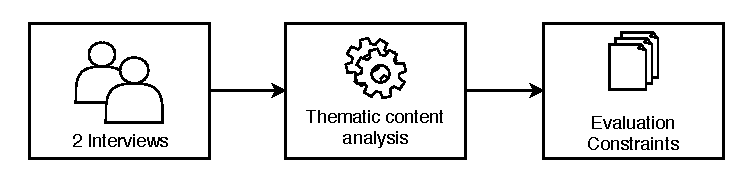
\includegraphics[width=\linewidth]{gfx/characterisation/constraintsIdentification}} \quad
\caption{Evaluation constraints identification process}\label{fig:constraintsIdentification}
\end{figure}

%-----------------------------------
\section{Constraints of evaluating PX in PREGs}\label{sec:constraints} % Findings ---------------
After transcribing interviews, we identified 69 statements regarding possible constraints of \acp{PREG}. Those statements were grouped into 4 final themes: patient related (38 statements), rehabilitation context (18 statements) and rehabilitation goal (13 statements). A summary of the findings is presented in \autoref{fig:constraintsGraph}. Regarding validation, the physiotherapist clarified or added information to five statements, this validation did not affect the resulting categories.

\begin{figure}[htb]
\myfloatalign
{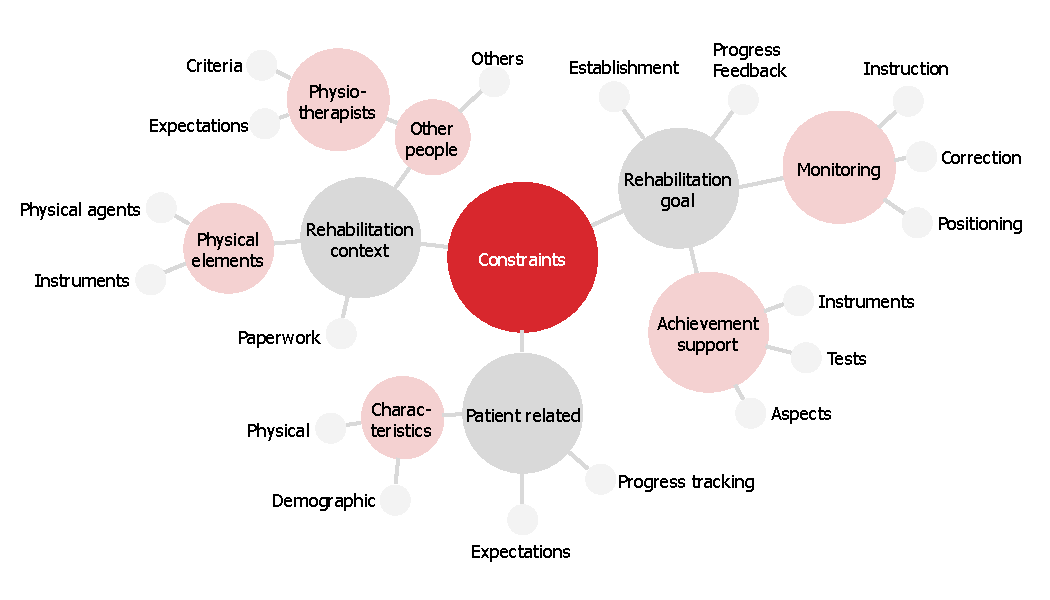
\includegraphics[width=\linewidth]{gfx/characterisation/constraintsGraph}} \quad
\caption{Map of qualitative findings, including themes and sub-themes associated to the constraints of \acp{PREG}}\label{fig:constraintsGraph}
\end{figure}

\acp{PREG} constraints are related to the \textit{rehabilitation environment} and \textit{goals} and the limitations imposed by the \textit{players' characteristics}. 

\subsection{Rehabilitation goal constraints}
\label{sec:reh_goal_constraints}
The physiotherapists indicated the importance of establishing rehabilitation goals to guide the whole physical rehabilitation process. They said that patients are evaluated in the first therapy session to set therapy goal(s) and a treatment plan. Patients are re-evaluated along the treatment to adapt therapy according to their progress.

They remarked that \acp{PREG} should be oriented to specific goals such as motion recovery, functional independence, motor coordination or proprioception.

The physiotherapists said that they assess the achievement of goals based on aspects associated with motion recovery and functional independence gain (e.g., range of motion and strength) by using physiotherapy instruments and methods (e.g., \ac{FIM}).

They highlighted that the feedback provided to patients should inform their performance during a therapy session. They provide continuous feedback and guidance to patients to guarantee the correct execution of exercises.

Also, physiotherapists provide feedback about overall patients' progress regarding rehabilitation goal(s). Additionally, the physiotherapists remarked that progress information is key to adapt therapy effectively.

\subsection{Rehabilitation context constraints}
\label{sec:reh_context_constraints}
According to the interviewees, the patients' opportunity to use a \ac{PREG} may depend on the physiotherapists' criteria. They are responsible for the patients' safety, and the inclusion of \acp{PREG} in a treatment may depend on patients' condition.

Furthermore, physiotherapists expect \acp{PREG} to assist their job, thereby being a supporting tool that does not increase the amount of workload that they already have. They think that a \ac{PREG} could bring dynamism and variety to the therapy.

Regarding the duration of a therapy session, they expressed that it usually lasts one hour, and they should plan what to include in each session carefully to achieve the expected goals.

In addition to physiotherapists, other people (e.g., rehabilitation assistants and other patients) may participate in or interrupt therapy sessions. Also, assisting objects such as weights and balls are used during therapy sessions to support the achievement of a therapeutic goal.

Finally, a physiotherapist expressed that the paperwork imposed by health institutions can affect the patients' motivation to start a rehabilitation treatment.

\subsection{Patient related constraints}
\label{sec:reh_patients_constraints}
The physiotherapists mentioned some of the common impairments that physiotherapy patients suffer, including lower and upper limbs fractures, cerebral palsy and lumbar pain. They remarked that \acp{PREG} could be used if patients are highly independent to avoid risks. Also, \acp{PREG} should not require patients to perform something they are not able to.

They remarked that treatments and \acp{PREG} should adapt to the physical characteristics of target patients to achieve rehabilitation goals safety. For instance, adults cannot play on unstable surfaces like a balance board. Similarly, they highlighted that \acp{PREG} should allow working on specific joints.

Furthermore, they highlighted that treatments might differ depending on demographic characteristics of patients such as age or literacy. For instance, adults require constant monitoring and reinforcement, whereas teenagers understand instructions easily and require less monitoring elderly.

Although the physiotherapists did not explicitly attribute motivation as one of their tasks, they mentioned what motivates or demotivates patients. Patients' major expectation is to progress and complete their treatments as soon as possible. Also, some causes for patients' lack of motivation are the monotony of exercises, pain, difficulty to perform an exercise or feeling that an activity does not contribute to the rehabilitation goal achievement. If a patient notice progression, he/she gets motivated, participates more and requests more challenging exercises; otherwise, he/she gets discouraged and tends to quit therapy.

% -----------------------------------------------
\section{Discussion}\label{sec:discussion_char} % Discussion -----------------------------------------------
Our findings suggest that \ac{PX} in \acp{PREG} should be evaluated considering constraints imposed by the sought after rehabilitation goal, the rehabilitation context; i.e. physiotherapists and other people intervention, and the patients' condition. Moreover, each \ac{PREG} may have additional constraints derived from the context of use and design that evaluators should identify when planning an evaluation.

In this section, we present the implications that the identified constraints may represent when evaluating \ac{PX} in \acp{PREG}.

\subsection{Rehabilitation goal constraints}
According to the physiotherapists' comments, and as suggested by \textcite{PirovanoAdvisor2012} the effectiveness of a \ac{PREG} may be assessed by its capability to assist the achievement of a rehabilitation goal. Thus, evaluators should assess aspects associated to movement execution such as amplitude, accuracy or speed. As expected, such assessment may require using clinical tests and instruments, as others evaluators have done \autocite{Brokaw2015,Burke2009,Cameirao2010,jansen2013serious,Ni2014,Seo2016,Wuest2014}. Consequently, physiotherapists may play an important role in evaluating a \ac{PREG} since they can decide and assess the aspects that may indicate its effectiveness.

Evaluators should concentrate on assessing if a \ac{PREG} meets the requirements to be used as part of a therapy. In early development stages, they may assess if the design process is focused on a rehabilitation goal \autocite{PirovanoAdvisor2012,Wiemeyer2015}; i.e., if the game mechanics relate directly to a set of movements and, as suggested by the physiotherapists, if the exercises can be configured to personalise the experience according to patients' needs \autocite{Ni2014,Nijholt2008,Wiemeyer2015}. Similarly, they must evaluate if a \ac{PREG} can be used safely by patients.

Moreover, they should assess the quality of the feedback provided by the \ac{PREG}. Patients need continuous information about rehabilitation progress and exercise correctness. It would allow physiotherapists making decisions based on rehabilitation goal achievement and keeping patients motivated. Also, evaluators should assess if interaction devices offer a point of view that allows patients to have a clear understanding of the outcome of  their actions \autocite{PirovanoAdvisor2012}; e.g., a third person view is more appropriate than a first person view, and big output screens might be preferred if patients are located at a certain distance from the devices.

Rehabilitation goal constraints should be considered before, during and after a player plays a \ac{PREG}. Before, those constraints require evaluators to assess if a \ac{PREG} supports a rehabilitation goal and if it is safe for patients considering aspects such as therapeutic goal centred design and configuration. During and after the interaction, evaluators would consider \ac{PX} from the therapeutic point of view regarding the performance and progress feedback, monitoring, adaptation and point of view.

\subsection{Rehabilitation context constraints}
When evaluating \acp{PREG} the participation of patients and physiotherapists may be required since they represent end users. Additionally, supervision of physiotherapists during evaluation sessions is always required to assure patients' safety \autocite{Wiemeyer2015}, as the physiotherapists expressed, they are responsible for patients' wellbeing. Therefore, they are the ones who can decide whether a patient could participate in an evaluation session or not. Consequently, evaluators should consider that the physiotherapists' participation may alter the interaction between a \ac{PREG} and a patient.  Also, evaluation logistics, such as time, number of participants, duration and location will depend on the internal regulations of health institutions. Furthermore, \acp{PREG} should meet physiotherapists' needs and expectations since they decide if a \ac{PREG} can be included in a therapy.

The physiotherapists expressed that the rehabilitation context may bring distractions to patients. Therefore, evaluators should assess aspects such as immersion and absorption \autocite{Lapas2015}. Additionally, the \ac{PREG}'s cognitive load should not distract patients from the expected rehabilitation goal \autocite{Isbister2015,Sinclair2007}. Also, interaction devices should enable the use of objects such as balls or weights if required by physiotherapists.

We also identified that time is an important aspect for physiotherapists. A \ac{PREG} should allow them to set the play session time as needed; e.g., 5 to 10 minutes for warming up, 20 for stimulus and 5 for cooling down \autocite{Sinclair2007}.

The physiotherapists mentioned that the patients' motivation is sometimes affected by the regulations of health institutions. For instance, some patients decide to stop attending their treatments due to the amount of paperwork they must complete before and during a therapy. Although patients' motivation towards their therapy is one of our main interests, we believe that it is out of the scope of \acp{PREG}. That indicates that there are contextual influences that go beyond the limits of patients, physiotherapists or \acp{PREG}.

Rehabilitation context constraints should be considered mainly before and during a player plays a \ac{PREG}. Before, these constraints may allow determining if a \ac{PREG} can be included in a therapy according to the physiotherapist's criteria. During the interaction, the presence of other people and objects should be assessed regarding their impact on \ac{PX}.

\subsection{Patient related constraints}
Physiotherapists expressed that some patients could not use a \ac{PREG}. Consequently, evaluators should define target participants including their physiological and physical characteristics. In that process, physiotherapists should be involved as source of information and Persona modelling might be employed \autocite{Mader2012}. Also, initial evaluations should involve healthy subjects, e.g. physiotherapists \autocite{Chu2011}, since patients safety has to be guaranteed.

Regarding adaptation to patient's needs, evaluators should assess if a \ac{PREG} can be configured before a play session to meet his/her characteristics \autocite{Ni2014,Nijholt2008,PirovanoAdvisor2012,Rego2018,Sinclair2007,Wiemeyer2015}. Also, they should assess if the \ac{PREG} adapts to patients' performance during interaction \autocite{PirovanoAdvisor2012,Rego2018}. Moreover, the correctness of exercise execution must be assured \autocite{Isbister2015,PirovanoAdvisor2012}, and patient's fatigue and over-exercise should be avoided \autocite{Isbister2015,Pasch2009,Zhang2011}.

Since patients have different demographic characteristics (e.g., age and literacy). \acs{PREG} should be easy to use and include tutorials or on-boarding levels. Additionally, \acp{PREG} should balance game challenges and patient's physical skills \autocite{Sinclair2007} and input devices should be natural and easy to use.

Patients' expectations are a source of motivation for them to continue playing in the future and achieve the expected rehabilitation goals. Thus, those expectations should be met by \acp{PREG}. The major expectation of adult patients is that \acp{PREG} contribute to their recovery process, in that case, if patients believe that a \ac{PREG} does not contribute to their early recovery, they may not want to play them. Therefore, evaluators may assess aspects such as proven clinical effectiveness, clinical feedback, \autocite{Seo2016} satisfaction \autocite{Sanchez2009,Yanez-Gomez2017,Zhao2016} and acceptance \autocite{Yanez-Gomez2017}. Meanwhile, the physiotherapists remarked that children prefer interactive activities. In that case, evaluators should assess if a \ac{PREG} offers an engaging and compelling experience \autocite{PirovanoAdvisor2012,Sinclair2007}.

Patients' related constraints should be considered before, during and after a player interacts with a \ac{PREG}. Before, those constraints may allow determining if a patient can use a \ac{PREG} as part of his/her therapy according to his/her condition and motivation towards it. During the interaction, evaluators should asses the experience of the patient regarding their motivations and attitudes. Finally, after the interaction, they should assess satisfaction and rehabilitation progress.

\subsection{Additional properties to characterise a \ac{PREG}}
Based on our findings, we argue that the following properties are relevant to characterise a \ac{PREG}. These properties may be complementary to those presented in  \autocite{Rego2018} and in \autoref{sec:characterising} since these are specifically for \acp{PREG} and are derived from the information provided by the interviewed physiotherapists.

\subsubsection{Associated movements}
The physiotherapists expressed that they need to work on particular joints depending on patients' needs. Although other works  \autocite{PirovanoAdvisor2012,Rego2018} include body parts (e.g. upper-limb, lower-limb and trunk), it may be relevant for physiotherapists to know exactly which movements are supported by a \ac{PREG} to include it in a rehabilitation treatment Also, associated movements should be directly related to game mechanics; i.e., they should enable game interaction.

\subsubsection{Associated configuration parameters}
The physiotherapists claimed that \acp{PREG} should meet patients' needs. That is, PGREs should be configurable to personalise game sessions for each patient. The configuration parameters should be related to the associated movements and the duration of a game session; e.g., movements or joints to be enabled, expected minimum and maximum range of motion, speed, number of repetitions and session time.

\subsubsection{Rehabilitation goals}
As discussed above, the mechanics of a \ac{PREG} should be guided by rehabilitation goals. Such goals may be generic (e.g. to increase the range of motion of shoulders extension) and must be set by, or in collaboration with, physiotherapists.

\subsubsection{Associated clinical instruments}
Physical rehabilitation instruments allow evaluators to assess the capability of a \ac{PREG} to assist the achievement of the associated rehabilitation goals. Those instruments include strength scales, balance tests and goniometer.

\subsubsection{Associated impairment}
This property is relevant for \acp{PREG} developed for a specific impairment; e.g., the ones presented in \autocite{Brokaw2015,Ni2014}. Knowing if a \ac{PREG} has an associated impairment may facilitate the work of a physiotherapist; e.g., when selecting a proper \ac{PREG} for a patient.

\subsection{Limitations}
Our findings cannot be generalised since the study was qualitative and we collected information from five interviews. Also, that information is based on the experience of the interviewees as physiotherapists. Their answers were based on their daily work at the hospital and their expectations and ideas regarding \acp{PREG}. They considered \acp{PREG} as a complementary tool and not as an autonomous therapy alternative. Consequently, most of the identified constraints apply to supervised \acp{PREG}; and another kind of study could be useful to identify additional constraints in the case of autonomous \acp{PREG}.

We could not include patients in our study due to availability reasons. Although the interviews with physiotherapists offered us new insights in the evaluation of \ac{PX} in \acp{PREG}, we consider that the set of constraints may be enriched by including the point of view of patients.

% -----------------------------------------------
\section{Conclusion}\label{sec:conclusion_char} % Conclusion -----------------------------------------------
We conducted a qualitative study to identify the constraints that evaluators should address when assessing \ac{PX} in a \ac{PREG}. Our results indicate that its use depends on physiotherapists' criteria and expectations, patients' expectations and its capability to assist the therapy.  We found that those constraints are related to three aspects: the sought after rehabilitation goal, the rehabilitation context and the patients' characteristics. Our findings allow us to conclude that a \ac{PREG} should be evaluated in terms of its capability to assist a rehabilitation goal and to motivate physiotherapists and patients to start and continue using them. Consequently, the methods employed to evaluate entertainment exergames should be extended to perform a relevant \ac{PX} evaluation since evaluators should consider the therapeutic purpose of \acp{PREG}. Our work contributes to a more comprehensive understanding of \acp{PREG} considering their context of use and their purpose as therapy. The results of this study may serve as the basis for the formulation of a model for \ac{PX} evaluation in \acp{PREG}. As expected, our results cannot be generalised since our study was completely qualitative.
